\documentclass{siamart1116}

% basics
\usepackage[left=3cm,right=3cm,top=3cm,bottom=4cm]{geometry}
\usepackage[utf8x]{inputenc}
\usepackage[title,titletoc]{appendix}
\usepackage{afterpage}
\usepackage{enumitem}   
\setlist[enumerate]{topsep=3pt,itemsep=3pt,label=(\roman*)}

% maths
\usepackage{mathtools}
\usepackage{amsmath}
\usepackage{amssymb}
\newsiamremark{assumption}{Assumption}
\newsiamremark{remark}{Remark}
\newsiamremark{example}{Example}
\numberwithin{theorem}{section}

% plots
\usepackage{pgfplots} 
\usepackage{graphicx}
\usepackage{tikz}
\usetikzlibrary{arrows.meta}
\usetikzlibrary{patterns}
\usepackage{subcaption}
\usepackage{here}
\usepackage[labelfont=bf]{caption}
\usepackage{xcolor}
\colorlet{light gray}{gray!40}

% tables
\usepackage{booktabs}

% title and authors
\newcommand{\TheTitle}{Invariant sets and measures: a short survey} 
\newcommand{\TheAuthors}{A. Abdulle, G. Garegnani}
\headers{Invariant sets and measures: a short survey}{\TheAuthors}
\title{{\TheTitle}}
\author{Assyr Abdulle\thanks{Mathematics Section, \'Ecole Polytechnique F\'ed\'erale de Lausanne (\email{assyr.abdulle@epfl.ch})}
	\and
	Giacomo Garegnani\thanks{Mathematics Section, \'Ecole Polytechnique F\'ed\'erale de Lausanne (\email{giacomo.garegnani@epfl.ch})}}

% my commands 

\DeclarePairedDelimiter{\ceil}{\left\lceil}{\right\rceil}
\DeclarePairedDelimiter{\floor}{\lfloor}{\rfloor}
\DeclarePairedDelimiter{\abs}{\lvert}{\rvert}
\DeclarePairedDelimiter{\norm}{\|}{\|}
\renewcommand{\phi}{\varphi}
\newcommand{\epl}{\varepsilon}
\newcommand{\eqtext}[1]{\ensuremath{\stackrel{#1}{=}}}
\newcommand{\leqtext}[1]{\ensuremath{\stackrel{#1}{\leq}}}
\newcommand{\iid}{\ensuremath{\stackrel{\text{i.i.d.}}{\sim}}}
\newcommand{\totext}[1]{\ensuremath{\stackrel{#1}{\to}}}
\newcommand{\ttt}{\texttt}
\newcommand{\N}{\mathbb{N}}
\newcommand{\R}{\mathbb{R}}
\newcommand{\C}{\mathbb{C}}
\newcommand{\OO}{\mathcal{O}}
\newcommand{\diffL}{\mathcal{L}}
\newcommand{\prior}{\mathcal{Q}}
\newcommand{\Borel}{\mathcal{B}}
\newcommand{\defeq}{\coloneqq}
\newcommand{\eqdef}{\eqqcolon}
\newcommand{\Var}{\operatorname{Var}}
\newcommand{\E}{\operatorname{\mathbb{E}}}
\newcommand{\MSE}{\operatorname{MSE}}
\newcommand{\trace}{\operatorname{tr}}
\newcommand{\sksum}{\textstyle\sum}
\newcommand{\dd}{\mathrm{d}}


\ifpdf
\hypersetup{
	pdftitle={\TheTitle},
	pdfauthor={\TheAuthors}
}
\fi

\begin{document}
	
\maketitle	

\begin{abstract}
\end{abstract}

\section{Introduction}

\section{Notation} Remark: the following notations and definitions summarize \cite{LaM94, DHJ97, EcR85}. Let us consider the function $f \colon \R^d \to \R^d$ and the autonomous ordinary differential equation (ODE)
\begin{equation}\label{eq:ODE}
\begin{aligned}
	y'(t) &= f(y(t)), \quad t > 0,\\
	y(0) &= y_0 \in \R^d. 	
\end{aligned}
\end{equation}
We consider $f$ to be Lipschitz continuous so that the solution of \eqref{eq:ODE} exists and we can define a family of mappings $\phi_t \colon \R^d \to \R^d$, for $t\geq 0$, such that
\begin{equation}\label{eq:ODEFlow}
	y(t) = \phi_t(y_0).
\end{equation}
Let us denote by $\Borel$ the $\sigma$-algebra of Borel sets in $\R^d$. For any set $B \in \mathcal{B}$, we denote then by $\phi_t^{-1}(B)$ the counterimage of $B$ through $\phi_t$, i.e., 
\begin{equation}
	\phi_t^{-1}(B) = \{x\in\R^d\colon \phi_t(x) \in B\}.
\end{equation}
Let us furthermore remark that if $f$ is Lipschitz, the mapping $\phi_t$ is measurable, i.e., $\phi_t^{-1}(B) \in \Borel$ for all Borel sets $B$. We now give some definitions and introduce notations useful for the following of our analysis.
\begin{definition} A set $B \in \Borel$ is invariant under the family $\{\phi_t\}_{t\geq 0}$ if 
	\begin{equation}
		\phi_t^{-1}(B) = B.
	\end{equation}
\end{definition}
We now denote by $\mathcal{M}$ the space of measures on $\R^d$.
\begin{definition} A measure $\mu \in \mathcal{M}$ on $(\R^d, \Borel)$ is said invariant for the dynamical system $\{\phi_t\}_{t\geq 0}$ if for all $B \in \Borel$ it holds
	\begin{equation}
		\mu(\phi^{-1}_t(B)) = \mu(B).
	\end{equation}
\end{definition}

\begin{definition} The operator $P\colon\mathcal{M}\to\mathcal{M}$ such that for all $B \in \Borel$ and $t \geq 0$
	\begin{equation}
		(P\mu)(B) = \mu(\phi^{-1}_t(B))
	\end{equation}
	is called the Frobenius-Perron operator. If $\{\phi_t\}_{t\geq 0}$ admits an invariant measure $\mu$, then it is trivially a fixed point of $P$, i.e., $P\mu = \mu$. 
\end{definition}
Given the definition of invariant sets and measure we can introduce the notion of ergodicity of a dynamical system.
\begin{definition} Given the measure space $(\R^d, \Borel, \mu)$, a dynamical system $\{\phi_t\}_{t\geq 0}$ is ergodic if for any invariant set $B \in \Borel$ it holds $\mu(B) = 0$ or $\mu(\R^d \setminus B) = 0$.
\end{definition}

\section{Exploring invariant sets and measures} We present two algorithms to explore the invariant set and measure of \eqref{eq:ODE}.
\subsection{Subdivision algorithm}
\begin{figure}[t]
	\begin{centering}
		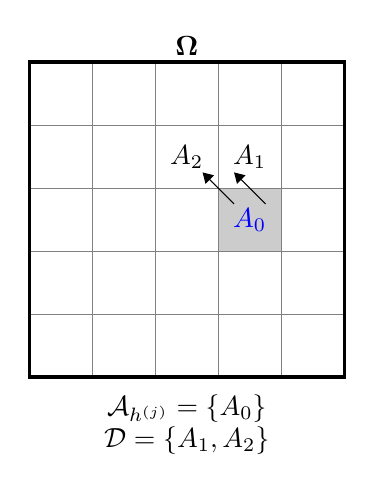
\begin{tikzpicture}[scale=2]
			\draw[step=0.4cm,color=gray,very thin] (0,0) grid (2.0,2.0);
			\draw[color=gray, very thin, fill = light gray] (1.2, 0.8) rectangle (1.6, 1.2);
			\node at (1.4, 1.0){\color{blue}$A_0$};
			\node at (1.4, 1.4){$A_1$};
			\node at (1.0, 1.4){$A_2$};
			\draw[-{Triangle[angle=60:1.5mm]}] (1.3, 1.1) -- (1.1, 1.3); 
			\draw[-{Triangle[angle=60:1.5mm]}] (1.5, 1.1) -- (1.3, 1.3);
			\node at (1.0, -0.2){$\mathcal{A}_{h^{(j)}} = \{A_0\}$};
			\node at (1.0, -0.4){$\mathcal{D} = \{A_1, A_2\}$};
			\node at (1.0, 2.1){$\boldsymbol{\Omega}$};
			\draw[color=black, very thick] (0, 0) rectangle (2.0, 2.0);
		\end{tikzpicture}
		\hspace{1.0cm}
		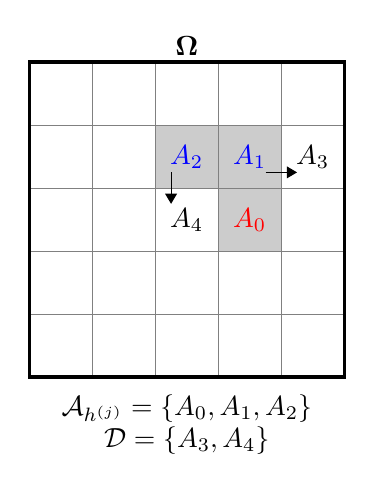
\begin{tikzpicture}[scale=2]
			\draw[step=0.4cm,color=gray,very thin] (0,0) grid (2.0,2.0);
			\draw[color=gray, very thin, fill = light gray] (1.2, 0.8) rectangle (1.6, 1.2);
			\draw[color=gray, very thin, fill = light gray] (0.8, 1.2) rectangle (1.2, 1.6);	
			\draw[color=gray, very thin, fill = light gray] (1.2, 1.2) rectangle (1.6, 1.6);
			\node at (1.4, 1.0){\color{red}$A_0$};
			\node at (1.4, 1.4){\color{blue}$A_1$};
			\node at (1.0, 1.4){\color{blue}$A_2$};
			\node at (1.8, 1.4){$A_3$};
			\node at (1.0, 1.0){$A_4$};
			\draw[-{Triangle[angle=60:1.5mm]}] (0.9, 1.3) -- (0.9, 1.1); 
			\draw[-{Triangle[angle=60:1.5mm]}] (1.5, 1.3) -- (1.7, 1.3);
			\node at (1.0, -0.2){$\mathcal{A}_{h^{(j)}} = \{A_0,A_1,A_2\}$};
			\node at (1.0, -0.4){$\mathcal{D} = \{A_3, A_4\}$};
			\node at (1.0, 2.1){$\boldsymbol{\Omega}$};
			\draw[color=black, very thick] (0, 0) rectangle (2.0, 2.0);
		\end{tikzpicture}
		\hspace{1.0cm}
		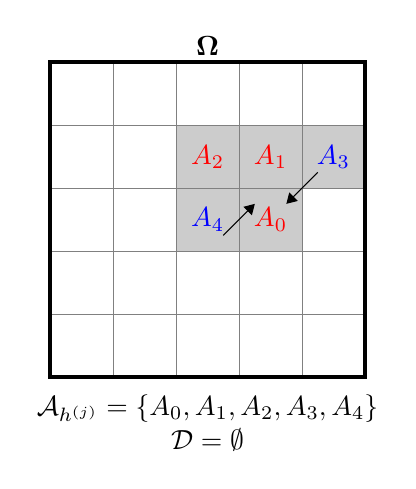
\begin{tikzpicture}[scale=2]
			\draw[step=0.4cm,color=gray,very thin] (0,0) grid (2.0,2.0);
			\draw[color=gray, very thin, fill = light gray] (1.2, 0.8) rectangle (1.6, 1.2);
			\draw[color=gray, very thin, fill = light gray] (0.8, 1.2) rectangle (1.2, 1.6);	
			\draw[color=gray, very thin, fill = light gray] (1.2, 1.2) rectangle (1.6, 1.6);
			\draw[color=gray, very thin, fill = light gray] (1.6, 1.2) rectangle (2.0, 1.6);	
			\draw[color=gray, very thin, fill = light gray] (0.8, 0.8) rectangle (1.2, 1.2);
			\node at (1.4, 1.0){\color{red}$A_0$};
			\node at (1.4, 1.4){\color{red}$A_1$};
			\node at (1.0, 1.4){\color{red}$A_2$};
			\node at (1.8, 1.4){\color{blue}$A_3$};
			\node at (1.0, 1.0){\color{blue}$A_4$};
			\draw[-{Triangle[angle=60:1.5mm]}] (1.1, 0.9) -- (1.3, 1.1); 
			\draw[-{Triangle[angle=60:1.5mm]}] (1.7, 1.3) -- (1.5, 1.1);
			\node at (1.0, -0.2){$\mathcal{A}_{h^{(j)}} = \{A_0,A_1,A_2,A_3,A_4\}$};
			\node at (1.0, -0.4){$\mathcal{D} = \emptyset$};
			\node at (1.0, 2.1){$\boldsymbol{\Omega}$};
			\draw[color=black, very thick] (0, 0) rectangle (2.0, 2.0);
		\end{tikzpicture}
		\caption{Graphical representation of the subdivision algorithm in a two-dimensional domain $\Omega$ under assumption \ref{ass:knownX0}. Fleshes indicate the action of the map $\phi_t$. The first square represents initialization, the second a step of the algorithm, while at the third square the algorithm is terminated.}
		\label{fig:AlgoSubdivision}
	\end{centering}
\end{figure} 

A method to approximate the invariant set of a dynamical system of the form \eqref{eq:ODE} has been presented in \cite{DHJ97}. We here report the main steps of the procedure. Given a vector with positive entries $r$ in $\R^d$ and a point $c$ in $\R^d$, we consider a rectangular domain $\Omega \in \R^d$, i.e., the set
\begin{equation}
	\Omega \defeq \{x \in \R^d \colon \abs{x_i - c_i} \leq r_i, \: i = 1, \ldots, d\},
\end{equation}
where $x_i$ is the $i$-th component of an element $x$ of $\R^d$. We denote in the following by $R_r(c)$ a rectangular domain as above. The method is based on the assumption that we have partial knowledge of the geometrical features of \eqref{eq:ODE}.
\begin{assumption} With the notation above, we assume that the domain $\Omega$ is chosen such that $B \subset \Omega$, where $B$ is an invariant set of \eqref{eq:ODE}.
\end{assumption}
Given a spatial discretization parameter $h > 0$, the goal is building a collection of non-overlapping rectangles $\mathcal{A}_h$ such that
\begin{enumerate}
	\item $\mathcal{A}_h = \{A_i \colon A_i = R_r(c_i), \text{ where } \norm{r}_{l^\infty} \leq h, \: c_i \in \Omega, \: A_i \cap A_j = \emptyset \text{ for } i \neq j\}_{i = 1}^N$,
	\item $B \subset \bigcup_{A \in \hat{\mathcal{A}}_{h^{(j+1)}}} A$,
	\item $\mathcal{A}_h \to B$ for $h \to 0$.
\end{enumerate}
In order to build such a set, we consider the following iterative procedure on the discretization parameter. Given $\mathcal{A}_{h^{(0)}} = \{\Omega\}$, and assuming that we have the collection $\mathcal{A}_{h^{(j)}}$ at the $j$-th step we proceed as follows
\begin{enumerate}
	\item Build a refined collection $\hat{\mathcal{A}}_{h^{(j+1)}}$ from $\mathcal{A}_{h^{(j)}}$ such that $h^{(j+1)} \leq h^{(j)}$ and 
		\begin{equation*}
			\textstyle \bigcup_{A \in \hat{\mathcal{A}}_{h^{(j+1)}}} A = \bigcup_{A \in \mathcal{A}_{h^{(j)}}} A.
		\end{equation*}
	\item Determine $\mathcal{A}_{h^{(j+1)}} \subset \hat{\mathcal{A}}_{h^{(j+1)}}$ selecting the sets that are mapped by $\phi_t$, i.e.,
		\begin{equation*}
			\mathcal{A}_{h^{(j+1)}} = \{A \in \hat{\mathcal{A}}_{h^{(j+1)}} \colon \phi_t^{-1}(A) \cap \hat A \neq \emptyset \text{ for some } \hat A \in \hat{\mathcal{A}}_{h^{(j+1)}}\}.
		\end{equation*}
\end{enumerate}
It has been shown that if $B$ is a global attractor for \eqref{eq:ODE} the sequence $\mathcal{A}_{h^{(j)}}$ satisfies
\begin{equation}
	\lim_{j\to\infty} d_{\text{H}}(\mathcal{A}_{h^{(j)}}, B) = 0,
\end{equation}
provided that the sequence $h_{j} \to 0$ for $j \to \infty$ and where $d_H(\cdot, \cdot)$ is the Hausdorff distance. If we have further knowledge of the geometrical properties of \eqref{eq:ODE}, it is possible to build $\mathcal{A}_{h^{(j)}}$ via a more effective scheme. 
\begin{assumption}\label{ass:knownX0} There exists a point $x_0$ in the domain $\Omega$ known \textit{a priori} such that $x \in B$, where $B$ is an attractor of \eqref{eq:ODE}.
\end{assumption}
Under this assumption, we can build $\mathcal{A}_{h^{(j)}}$ proceeding as follows:
\begin{enumerate}
	\item build a collection $\tilde{\mathcal{A}}_{h^{(j)}}$ such that $\bigcup_{A \in \tilde{\mathcal{A}}_{h^{(j)}}} A = \Omega$,
	\item find the element $A$ of $\tilde{\mathcal{A}}_{h^{(j)}}$ such that $x_0 \in A$ and denote it as $A_0$, then $\mathcal{A}_{h^{(j)}} = \{A_0\}$,
	\item\label{item:startofloop} choose a set of points $\{x_i\}_{i=1}^M$ inside $A_0$ and compute the mapped points $\{y_i = \phi_t(x_i)\}_{i=1}^M$,
	\item find the smallest subset $\mathcal{D}$ of $\tilde{\mathcal{A}}_{h^{(j)}}$ such that $y_i \in \bigcup_{A \in \mathcal{D}} A$  for all $i = 1, \ldots, d$,
	\item\label{item:endofloop} update $\mathcal{A}_{h^{(j)}} \leftarrow \mathcal{A}_{h^{(j)}} \cup \mathcal{D}$,
	\item for each of the elements of $\mathcal{D}$ not considered yet, proceed from \ref{item:startofloop} to \ref{item:endofloop},
	\item terminate when $\mathcal{D} = \emptyset$.
\end{enumerate}
A graphical representation of this algorithm is depicted in Figure \ref{fig:AlgoSubdivision}. 

Once a covering $\mathcal{A}_h$ of the attractor is known, it is possible to find an approximation $\mu_h$ of the density of the invariant measure $\mu$ of \eqref{eq:ODE} by a Galerkin method \cite{DHJ97}. In particular, we search $\mu_h$ in the space of densities of probability measure which are constant on each set $A$ in $\mathcal{A}_h$, i.e.,
\begin{equation}
\begin{aligned}
	\mu_h(x) &= \mu_i \in \R, && \forall x \in A_i, \: \forall A_i \in \mathcal{A}_h,\ \: i = 1, \ldots, \abs{\mathcal{A}_h},\\
	\int_{\bigcup_{A\in\mathcal{A}_h} A} \mu_h(x) \dd x &= 1, \\
	\mu_h(x) &= 0, && \forall x \in \Omega \setminus \textstyle \bigcup_{A\in\mathcal{A}_h} A.
\end{aligned}
\end{equation} 
In particular, if $\abs{\mathcal{A}_h} = n$, we can uniquely represent $\mu_h$ as a vector of $\R^n$. We obtain the approximation by recalling that for $P\mu = \mu$, where $P$ is the Frobenius-Perron operator. We approximate $P$ by a matrix $P_h \in \R^{n\times n}$ whose entries are given by
\begin{equation}
	(P_h)_{ij} = \frac{m(\phi_t^{-1}(A_i) \cap A_j)}{m(A_j)}, \quad \forall A_i, A_j \in \mathcal{A}_h,
\end{equation}
where $m$ is the Lebesgue measure. Then, we compute $\mu_h$ as the eigenvector of $P_h$ associated with the eigenvalue one, i.e.
\begin{equation}\label{eq:GalerkinFP}
	P_h \mu_h = \mu_h.
\end{equation}
Let us remark that the elements of $P_h$ are approximated in practice by a Monte Carlo average as
\begin{equation}
	(P_h)_{ij} \approx M^{-1} \sksum_{i = 1}^M \chi_{A_i}(\phi_t(x_i)),
\end{equation}
where the $M$ points $x_i$ are random samples from $A_j$. Finally, let us remark that due to the local interaction of the flow map, the matrix $P_h$ should be sparse.

\subsection{Probabilistic integrator approach} Let us consider \eqref{eq:ODE} and a probabilistic numerical solution $Y_N$ taking values in $\R^d$ obtained either with the additive noise technique \cite{CGS16} or with the random time-stepping scheme. We consider the random variable $Y_N$ to be an approximation of the solution $y(T)$ of \eqref{eq:ODE} at a sufficiently long time $T = N\Delta_t$, where $\Delta_t$ is the time step employed to obtain the numerical solution.

We approximate the density $\mu_h$ of the invariant measure using samples $Y_N^{(i)}$, $i = 1, \ldots, M$, drawn from the random variable $Y_N$. In particular, we exploit a kernel density estimation, i.e., for each value $x \in \R^d$ we consider the estimator $\hat \mu_h(x)$ given by
\begin{equation}
\hat \mu_h(x) = M^{-1}\sksum_{i=1}^{M} K(x - Y_N^{(i)}).
\end{equation}
The function $K\colon\R^d\to\R$ is a Gaussian kernel given by 
\begin{equation}
K(x) = (2\pi)^{(-d/2)}\det(H)^{(-1/2)}e^{-x^TH^{-1}x/2},
\end{equation}
where the covariance bandwidth $H$ is a diagonal matrix of $\R^{d\times d}$ whose entries are chosen with Silverman's rule of thumb \cite{Sil86}, i.e.,
\begin{equation}
H_{i,i}^{1/2} = \Big(\frac{4}{n(d + 2)}\Big) ^ {1 / (d + 4)} \sigma_i,
\end{equation}
and where $\sigma_i$ are the component-wise population standard deviations of the chosen draws.

\section{Numerical experiments} 
We show numerical experiments of the procedures discussed in the above section. The computations are carried out with a self-developed \ttt{C++ / Matlab} code.
\subsection{Subdivision algorithm} 
\begin{figure}[t]
	\begin{center} 
		\begin{subfigure}[b]{0.49\textwidth}
			\includegraphics[width=\linewidth]{BoxesFitznag}
			\caption{Collection $\mathcal{A}_h$, coarse grid.}
			\label{fig:FitzNagBoxesA}
		\end{subfigure}	
		\begin{subfigure}[b]{0.49\textwidth}
			\includegraphics[width=\linewidth]{BoxesFitznagDens}
			\caption{Approximation $\mu_h$, coarse grid.}
			\label{fig:FitzNagBoxesB}
		\end{subfigure}
		\begin{subfigure}[b]{0.49\textwidth}
			\includegraphics[width=\linewidth]{BoxesFitznagDensZoom}
			\caption{Approximation $\mu_h$, fine grid, zoom.}
			\label{fig:FitzNagBoxesC}
		\end{subfigure} 
	\end{center}
	\caption{Approximation of the attractor $A$ of \eqref{eq:FitzNag} and of the density of the invariant measure $\mu$.}
	\label{fig:FitzNagBoxes}
\end{figure}

We first consider the FitzHug-Nagumo ODE, which reads
\begin{equation}\label{eq:FitzNag}
\begin{aligned}
	y_1' &= c\Big(y_1 - \frac{y_1^3}{3} + y_2\Big), && y_1(0) = -1, \\
	y_2' &= -\frac{1}{c}(y_1 - a + by_2), && y_2(0) = 1,
\end{aligned}
\end{equation}
where $a, b, c$ are real parameters with values $a = 0.2$, $b = 0.2$, $c = 3$. It is known that with these values for the parameters, the equation admits a limit cycle. We then perform the subdivision algorithm starting from a point laying close to the limit cycle to obtain an approximation $\mathcal{A}_h$ of the attractor $A$ and compute the invariant density with \eqref{eq:GalerkinFP}. In Figure \ref{fig:FitzNagBoxesA} and \ref{fig:FitzNagBoxesB}, we can see the result obtained with a coarse discretization index $h$ of $\mathcal{A}_h$. In Figure \ref{fig:FitzNagBoxesC} we can see that results are smoother in case of a finer discretization. 

We now consider a three-dimensional model, the Lorenz equations, which is of particular interest. The ODE reads
\begin{equation}\label{eq:Lorenz}
\begin{aligned}
	y_1' &= \sigma(y_2 - y_1), \quad &&y_1(0) = -10,\\
	y_2' &= y_1(\rho - y_3) - y_2, \quad &&y_2(0) = -1,\\
	y_3' &= y_1y_2 - \beta y_3, \quad &&y_3(0) = 40.
\end{aligned}
\end{equation}
with parameters values. $\sigma = 10$, $\rho = 28$, $\beta = 8/3$. It has been shown \cite{LOR63} that with these values for the parameters, the solution of \eqref{eq:Lorenz} has a chaotic behavior. Nonetheless, the system admits a strange attractor $A$ and a unique invariant measure $\mu$ with support on $A$ \cite{Tuc99, HoM07}. In Figure \ref{fig:LorenzBoxes} we show the results for the density estimation on the collection of boxes $\mathcal{A}_h$. The computational time is quite low even in a three-dimensional problem. In this case, we generated 2827 boxes, so the matrix $P_h$ has 7991929 elements. However, storage is not an issue as $P_h$ has only 40180 non-zero entries, thus confirming our hypothesis that $P_h$ should be sparse.

\begin{figure}[t]
	\begin{center} 
		\includegraphics[width=0.6\linewidth]{BoxesLorenzDens}
	\end{center}
	\caption{Approximation of the density of the invariant measure $\mu$ for the Lorenz equation with the subdivision method.}
	\label{fig:LorenzBoxes}
\end{figure}

\section{Probabilistic integrator} We consider equation \eqref{eq:Lorenz} and draw samples from both the additive noise model \cite{CGS16} and with the random time-stepping integrator. We then estimate the density with the kernel estimator, using as evaluation points the draws themselves. Results (Figure \ref{fig:LorenzStepAdd}) show that the random time-stepping and the additive noise methods are consistent, producing similar density estimations. It is possible to remark that the shape of the attractor and the order of magnitude of the density are comparable with respect to the results provided by the subdivision method.
 
\begin{figure}[t]
	\begin{center} 
		\begin{subfigure}[b]{0.49\textwidth}
			\includegraphics[width=\linewidth]{StepLorenzDens}
			\caption{Random time-stepping.}
		\end{subfigure}	
		\begin{subfigure}[b]{0.49\textwidth}
			\includegraphics[width=\linewidth]{AddLorenzDens}
			\caption{Additive noise.}
		\end{subfigure} 
	\end{center}
	\caption{Approximation of the density of the invariant measure $\mu$ for the Lorenz equation with the probabilistic integrator for ODEs.}
	\label{fig:LorenzStepAdd}
\end{figure}

\bibliographystyle{siamplain}
\bibliography{anmc}

\end{document}